
%(BEGIN_QUESTION)
% Copyright 2003, Tony R. Kuphaldt, released under the Creative Commons Attribution License (v 1.0)
% This means you may do almost anything with this work of mine, so long as you give me proper credit

Write the transfer function (input/output equation) for an operational amplifier with an open-loop voltage gain of 100,000, and the inverting input connected directly to its output terminal.  In other words, write an equation describing the output voltage of this opamp ($V_{out}$) for any given input voltage at the noninverting input ($V_{in(+)}$):

$$\includegraphics[width=15.5cm]{i01472x01.eps}$$

Then, once you have an equation written, solve for the over-all voltage gain ($A_V = {V_{out} \over V_{in(+)}}$) of this amplifier circuit, and calculate the output voltage for a noninverting input voltage of +6 volts.

\underbar{file i01472}
%(END_QUESTION)





%(BEGIN_ANSWER)

$$V_{out} = 100,000(V_{in(+)} - V_{out})$$

(I've left it up to you to perform the algebraic simplification here!)

$$A_V = {100,000 \over 100,001} = 0.99999$$

\vskip 10pt

For an input voltage of +6 volts, the output voltage will be +5.99994 volts.

\vskip 10pt

Follow-up question: how much will the closed-loop gain ($\approx$ 1) be affected by large changes in the opamp's internal voltage gain of 100,000?

%(END_ANSWER)





%(BEGIN_NOTES)

The significant point of this question is that students see the over-all voltage gain of the opamp radically attenuated from 100,000 to approximately 1.  What is not so evident is just how {\it stable} this new voltage gain is, which is one of the purposes for employing negative feedback.

%INDEX% Electronics review: opamp buffer gain calculation (precise)

%(END_NOTES)


